%iffalse%\let\negmedspace\undefined
\let\negthickspace\undefined
\documentclass[journal,12pt,onecolumn]{IEEEtran}
\usepackage{cite}
\usepackage{amsmath,amssymb,amsfonts,amsthm}
\usepackage{algorithmic}
\usepackage{graphicx}
\usepackage{textcomp}
\usepackage{xcolor}
\usepackage{txfonts}
\usepackage{listings}
\usepackage{enumitem}
\usepackage{mathtools}
\usepackage{gensymb}
\usepackage{comment}
\usepackage[breaklinks=true]{hyperref}
\usepackage{tkz-euclide} 
\usepackage{listings}
\usepackage{gvv}                                        
%\def\inputGnumericTable{}                                 
\usepackage[latin1]{inputenc}     
\usepackage{xparse}
\usepackage{color}                                            
\usepackage{array}                                            
\usepackage{longtable}                                       
\usepackage{calc}                                             
\usepackage{multirow}
\usepackage{multicol}
\usepackage{hhline}                                           
\usepackage{ifthen}                                           
\usepackage{lscape}
\usepackage{tabularx}
\usepackage{array}
\usepackage{float}
\newtheorem{theorem}{Theorem}[section]
\newtheorem{problem}{Problem}
\newtheorem{proposition}{Proposition}[section]
\newtheorem{lemma}{Lemma}[section]
\newtheorem{corollary}[theorem]{Corollary}
\newtheorem{example}{Example}[section]
\newtheorem{definition}[problem]{Definition}
\newcommand{\BEQA}{\begin{eqnarray}}
\newcommand{\EEQA}{\end{eqnarray}}
\usepackage{float}
%\newcommand{\define}{\stackrel{\triangle}{=}}
\theoremstyle{remark}
\usepackage{ circuitikz }
%\newtheorem{rem}{Remark}
% Marks the beginning of the document


\begin{document}

\title{GATE 2024-BM}
\author{EE25BTECH11015 - Bhoomika V}
\maketitle
\renewcommand{\thefigure}{\theenumi}
\renewcommand{\thetable}{\theenumi}

\maketitle{GA-General Aptitude}\\

% (add your content here)
\noindent \textbf{Q. 1 --Q.  \textbf{5}} carry ONE mark each
\begin{enumerate}

\item If `$\rightarrow$' denotes increasing order of intensity, then the meaning of the words  

\[
[\text{simmer} \rightarrow \text{seethe} \rightarrow \text{smolder}]
\] is analogous to  \[
[\text{break} \rightarrow \text{raze} \rightarrow \_\_\_\_\_\_ ].
\]

Which one of the given options is appropriate to fill the blank? 
\begin{enumerate}[label=(\Alph*)] 
    \item obfuscate
    \item obliterate
    \item fracture
    \item fissure
\end{enumerate}
\hfill $\brak{GATE\ BM\ 2024}$

\item In a locality, the houses are numbered in the following way:\\

The house-numbers on one side of a road are consecutive odd integers starting from
301, while the house-numbers on the other side of the road are consecutive even
numbers starting from 302. The total number of houses is the same on both sides of
the road.\\

If the difference of the sum of the house-numbers between the two sides of the road
is 27, then the number of houses on each side of the road is
\begin{enumerate}[label=(\Alph*)] 
    \item 27
    \item 52
    \item 54
    \item 26
\end{enumerate}
\hfill $\brak{GATE\ BM\ 2040}$

\item For positive integers $p$ and $q$, with $\tfrac{p}{q} \neq 1$,  
\[
\left(\frac{p}{q}\right)^{\tfrac{p}{q}} = p^{\left(\tfrac{p}{q} - 1\right)}.
\]  
Then,  

\begin{enumerate}[label=(\Alph*)] 
    \item $q^p = p^q$
    \item $q^p = p^{2q}$
    \item $\sqrt{q} = \sqrt{p}$
    \item $\sqrt[p]{q} = \sqrt[q]{p}$
\end{enumerate}
\hfill $\brak{GATE\ BM\ 2024}$

\item Which one of the given options is a possible value of x in the following sequence?\\

3, 7, 15, x, 63, 127, 255\\
\begin{enumerate}[label=(\Alph*)] 
    \item 35 
    \item 40
    \item45
    \item31
\end{enumerate}
\hfill $\brak{GATE\ BM\ 2024}$

\item On a given day, how many times will the second-hand and the minute-hand of a
clock cross each other during the clock time 12:05:00 hours to 12:55:00 hours?
\begin{enumerate}[label=(\Alph*)] 
    \item 51
    \item49
    \item50
    \item55
\end{enumerate}
\hfill $\brak{GATE\ BM\ 2024}$

\item In the given text, the blanks are numbered (i)--(iv). Select the best match for all the blanks.  

\medskip

From the ancient Athenian arena to the modern Olympic stadiums, athletics \underline{(i)} the potential for a spectacle. The crowd \underline{(ii)} with bated breath as the Olympian artist twists his body, stretching the javelin behind him. Twelve strides in, he begins to cross-step. Six cross-steps \underline{(iii)} in an abrupt stop on his left foot. As his body \underline{(iv)} like a door turning on a hinge, the javelin is launched skyward at a precise angle.  

\medskip

\begin{enumerate}[label=(\Alph*)]
    \item (i) hold \quad (ii) waits \quad (iii) culminates \quad (iv) pivot
    \item (i) holds \quad (ii) wait \quad (iii) culminates \quad (iv) pivot
    \item (i) hold \quad (ii) wait \quad (iii) culminate \quad (iv) pivots
    \item (i) holds \quad (ii) waits \quad (iii) culminates \quad (iv) pivots
\end{enumerate}
\hfill $\brak{GATE\ BM\ 2024}$

\item Three distinct sets of indistinguishable twins are to be seated at a circular table that
has 8 identical chairs. Unique seating arrangements are defined by the relative
positions of the people.\\
\\How many unique seating arrangements are possible such that each person is sitting
next to their twin?
\begin{enumerate}[label=(\Alph*)]
    \item 12
    \item 14
    \item 10
    \item 28
\end{enumerate}
\hfill $\brak{GATE\ BM\ 2024}$    

\item The chart given below compares the Installed Capacity (MW) of four power generation technologies, T1, T2, T3, and T4, and their Electricity Generation (MWh) in a time of 1000 hours (h).  

\begin{figure}[H]
\centering
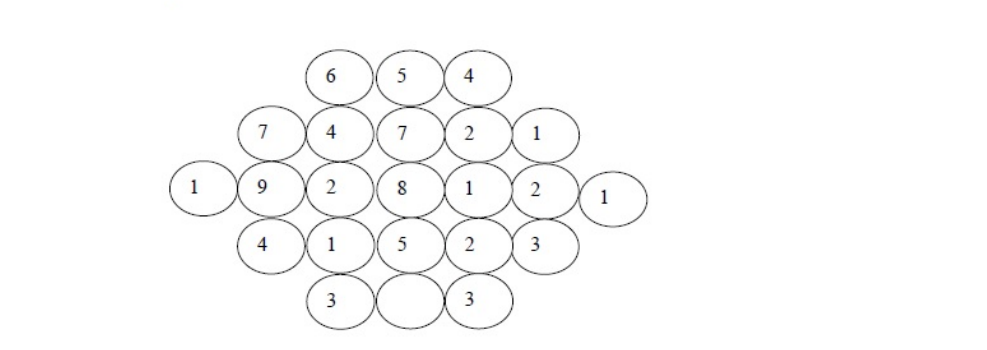
\includegraphics[width=0.4\columnwidth]{Figs/fig 1.png}
\caption{chart}
\label{fig:placeholder}
\end{figure}

The Capacity Factor of a power generation technology is:  

\[
\text{Capacity Factor} = \frac{\text{Electricity Generation (MWh)}}{\text{Installed Capacity (MW)} \times 1000 \, (\text{h})}
\]

Which one of the given technologies has the highest Capacity Factor? 
\begin{enumerate}[label=(\Alph*)]
    \item T1
    \item T2
    \item T3
    \item T4
\end{enumerate}    
\hfill $\brak{GATE\ BM\ 2024}$  

\item In the $4 \times 4$ array shown below, each cell of the first three columns has either a cross (X) or a number, as per the given rule.  

\[
\begin{array}{|c|c|c|c|}
\hline
1 & 1 & 2 &  \\ \hline
2 & X & 3 &  \\ \hline
2 & X & 4 &  \\ \hline
1 & 2 & X &  \\ \hline
\end{array}
\]

\textbf{Rule:} The number in a cell represents the count of crosses around its immediate neighboring cells (left, right, top, bottom, diagonals).  

As per this rule, the \textbf{maximum} number of crosses possible in the empty column is \underline{\hspace{2cm}}
\begin{enumerate}[label=(\Alph*)]
    \item 0
    \item 1
    \item 2
    \item 3
\end{enumerate}    
\hfill $\brak{GATE\ BM\ 2024}$     

\item During a half-moon phase, the Earth-Moon-Sun form a right triangle. If the
Moon-Earth-Sun angle at this half-moon phase is measured to be 89.85°, the ratio
of the Earth-Sun and Earth-Moon distances is closest to
\begin{enumerate}[label=(\Alph*)]
    \item 328
    \item 382
    \item 238
    \item 283
\end{enumerate}    
\hfill $\brak{GATE\ BM\ 2024}$ 

\item What is the value of the following complex line integral counter-clockwise?

\[
\oint_{|z|=3} \frac{8}{z(z-2)(z-4)} \, dz
\]

\begin{enumerate}[label=(\Alph*)]
\item $+j2\pi$
\item $-j2\pi$
\item $-j10\pi$
\item $+j10\pi$
\end{enumerate}
\hfill $\brak{GATE\ BM\ 2024}$ 

\item To solve the equation $x = 2\cos x$ using Newton-Raphson's method, which one of the following iterations should be used?

\begin{enumerate}[label=(\Alph*)]
\item $x_{n+1} = x_n - \dfrac{x_n - 2\cos x_n}{1 + 2\sin x_n}$
\item $x_{n+1} = x_n + \dfrac{x_n - 2\cos x_n}{1 + 2\sin x_n}$
\item $x_{n+1} = x_n + \dfrac{1 + 2\sin x_n}{x_n - 2\cos x_n}$
\item $x_{n+1} = x_n - \dfrac{1 + 2\sin x_n}{x_n - 2\cos x_n}$
\end{enumerate}
\hfill $\brak{GATE\ BM\ 2024}$ 

\item During the repolarization phase of a neuron, the cell is brought back to the resting
potential by the action of a Sodium-Potassium pump. Which one of the following
statements is  \textbf{TRUE} for the active transport of $Na^{+}$ and  $K^{+}$ ions through the cell
membrane?
\begin{enumerate}[label=(\Alph*)]
\item For every 3 $Na^{+}$ transported out of the cell 2 $K^{+}$ is transported into the cell.
\item For every 3 $Na^{+}$ transported into the cell 2 $K^{+}$ is transported out of the cell.
\item For every 2 $Na^{+}$ transported out of the cell 3 $K^{+}$ is transported into the cell.
\item The ratio of $Na^{+}$ and $K^{+}$ transport is always equal to one.
\end{enumerate}
\hfill $\brak{GATE\ BM\ 2024}$ 

\item The cardiac rhythm in a healthy human heart originates from  \underline{\hspace{2cm}}
\begin{enumerate}[label=(\Alph*)]
\item Sinu-atrial node (SA)
\item Atrio ventricular node (AV)
\item Aorta
\item Right atria
\end{enumerate}
\hfill $\brak{GATE\ BM\ 2024}$ 

\item Which one of the following events is \textbf{NOT} typically encountered in diagnostic
X-ray projection radiography?
\begin{enumerate}[label=(\Alph*)]
\item Pair production
\item Photoelectric absorption
\item Compton scattering
\item Characteristic radiation
\end{enumerate}
\hfill $\brak{GATE\ BM\ 2024}$

\item Which of the following statements is \textbf{TRUE} for a pet imaging system ?
\begin{enumerate}[label=(\Alph*)]
\item Two coincident photons of 511 keV energy are detected $180^\circ$. apart.
\item Photons of 51.1 keV energy are detected $360^\circ$. around the body.
\item Photons of energy 511 keV are detected $360^\circ$. around the body.
\item Coincident photons with 51.1 keV energy are detected $180^\circ$ apart.
\end{enumerate}
\hfill $\brak{GATE\ BM\ 2024}$

\item Consider the following layers: subcutaneous fat, viable epidermis, stratum
corneum, and dermis. Which one of the following represents the correct sequence
of the layers from skin surface to within? 
\begin{enumerate}[label=(\Alph*)]
\item Dermis, subcutaneous fat, viable epidermis, stratum corneum
\item Dermis, viable epidermis, subcutaneous fat, stratum corneum
\item Stratum corneum, viable epidermis, dermis, subcutaneous fat
\item Viable epidermis, stratum corneum, dermis, subcutaneous fat
\end{enumerate}
\hfill $\brak{GATE\ BM\ 2024}$

\item Bioglass 45S5 has a composition of \underline{\hspace{2cm}}. 
\begin{enumerate}[label=(\Alph*)]
\item 45 wt\% SiO$_2$ and 5:1 molar ratio of Calcium to Phosphorus. 
\item 45 wt\% Hydroxyapatite and 5 wt\% SiO$_2$.
\item 45 wt\% Hydroxyapatite and 5:1 molar ratio of CaO and Ca$_3$(PO$_4$)$_2$.
\item 45 wt\% SiO$_2$ and 5 wt\% Hydroxyapatite.
\end{enumerate}
\hfill $\brak{GATE\ BM\ 2024}$

\item Macrophages that are resident in the liver are \underline{\hspace{2cm}}
\begin{enumerate}[label=(\Alph*)]
\item Histiocyte cells
\item Langerhans cells
\item Kupffer cells
\item Fibroblast cells
\end{enumerate}
\hfill $\brak{GATE\ BM\ 2024}$

\item Which one of the following drug release kinetic curves will be ideal for developing an implantable slow-release drug delivery device? 
\begin{enumerate}[label=(\Alph*)]
\item 
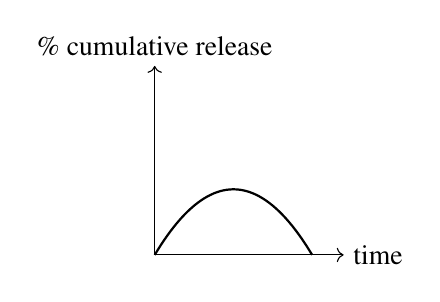
\begin{tikzpicture}[scale=0.8]
\draw[->] (0,0) -- (3,0) node[right]{time};
\draw[->] (0,0) -- (0,3) node[above]{\% cumulative release};
\draw[thick, domain=0:2.5, smooth] plot (\x, {2*\x*(2.5-\x)/3});
\end{tikzpicture}
\vspace{0.5cm}
\item 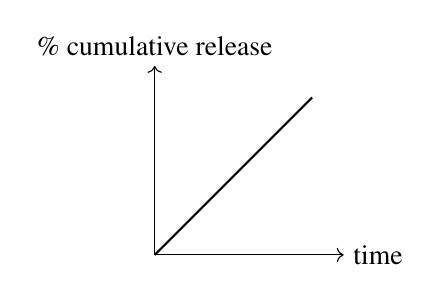
\begin{tikzpicture}[scale=0.8]
\draw[->] (0,0) -- (3,0) node[right]{time};
\draw[->] (0,0) -- (0,3) node[above]{\% cumulative release};
\draw[thick] (0,0) -- (2.5,2.5);
\end{tikzpicture}
\vspace{0.5cm}
\item 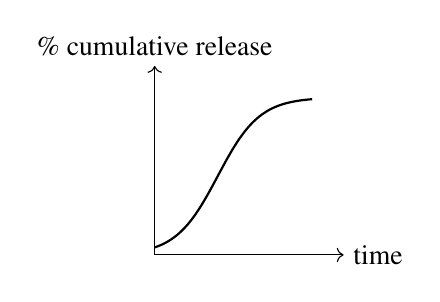
\begin{tikzpicture}[scale=0.8]
\draw[->] (0,0) -- (3,0) node[right]{time};
\draw[->] (0,0) -- (0,3) node[above]{\% cumulative release};
\draw[thick, domain=0:2.5, smooth] plot (\x, {2.5*(1/(1+exp(-(3*\x-3))))});
\end{tikzpicture}
\vspace{0.5cm}
\item 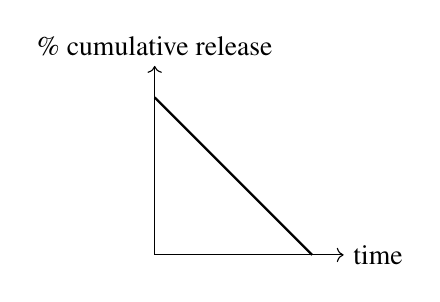
\begin{tikzpicture}[scale=0.8]
\draw[->] (0,0) -- (3,0) node[right]{time};
\draw[->] (0,0) -- (0,3) node[above]{\% cumulative release};
\draw[thick] (0,2.5) -- (2.5,0);
\end{tikzpicture}
\vspace{0.5cm}
\end{enumerate}
\hfill $\brak{GATE\ BM\ 2024}$

\item The circuit shown in the figure functions as which one of the following digital
circuit blocks?
\begin{figure}[H]
\centering
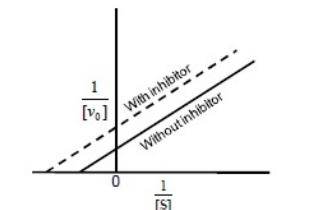
\includegraphics[width=0.2\columnwidth]{Figs/fig 2.png}
\caption{circuit}
\label{fig:placeholder}
\end{figure}
\begin{enumerate}[label=(\Alph*)]
\item Negative level triggered D-latch
\item Positive level triggered D-latch
\item Negative edge triggered D-flip-flop
\item Positive edge triggered D-flip-flop
\end{enumerate}
\hfill $\brak{GATE\ BM\ 2024}$

\item The Fourier transform of $e^{-2|t|}$ is \underline{\hspace{2cm}}.
\begin{enumerate}[label=(\Alph*)]
\item \quad $\dfrac{4}{4 - \omega^2}$ \\[10pt]
\item \quad $\dfrac{4}{4 + \omega^2}$ \\[10pt]
\item \quad $\dfrac{2}{2 + \omega}$ \\[10pt]
\item \quad $\dfrac{2}{2 - \omega}$
\end{enumerate}
\hfill $\brak{GATE\ BM\ 2024}$

\item The Bode plot of a $2^{nd}$ order low pass filter is shown in the figure below. What is the frequency at which the attenuation is 80 dB?
\begin{figure}[H]
\centering
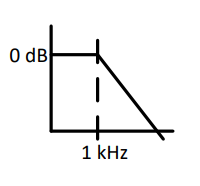
\includegraphics[width=0.4\columnwidth]{Figs/Fig 3.png}
\caption{plot}
\label{fig:placeholder}
\end{figure}
\begin{enumerate}[label=(\Alph*)]
\item 10 kHz
\item 10 MHz
\item 100 kHz
\item 100 MHz
\end{enumerate}
\hfill $\brak{GATE\ BM\ 2024}$

\item \quad The input $x(t)$ and the output $y(t)$ of a linear time invariant system are related as follows:  

\[
y(t) + \frac{dy(t)}{dt} + 0.5 \frac{d^2 y(t)}{dt^2} = x(t) + 0.1 \frac{dx(t)}{dt}
\]

\noindent What is the Laplace transform of the impulse response of the system? 
\begin{enumerate}[label=(\Alph*)]
\item \quad $\dfrac{0.5s^2 + s + 1}{0.1s + 1}$\\
\item \quad $\dfrac{0.1s + 1}{0.5s^2 + s + 1}$ \\
\item \quad $\dfrac{0.1s + s^2}{s^2 + s + 0.5}$\\ 
\item \quad $\dfrac{s^2 + s + 0.5}{0.1s^2 + s}$\\
\end{enumerate}
\hfill $\brak{GATE\ BM\ 2024}$

\item Match the different chambers/locations of a healthy human heart in Column-1 to the ranges of \textbf{diastolic} pressures in Column-2. \\[8pt]

\begin{tabular}{|c|c|c|}
\hline
 & \textbf{Column-1} & \textbf{Column-2} \\
\hline
(P) & Arterial          & (I) \; 2--6 mm Hg \\
(Q) & Pulmonary artery  & (II) \; 8--12 mm Hg \\
(R) & Right ventricle   & (III) \; 60--80 mm Hg \\
\hline
\end{tabular}
\vspace{1em}
\begin{enumerate}[label=(\Alph*)]
\item (P) -- (II), (Q) -- (III), (R) -- (I) 
\item (P) -- (II), (Q) -- (I), (R) -- (III) 
\item (P) -- (III), (Q) -- (II), (R) -- (I) 
\item (P) -- (III), (Q) -- (I), (R) -- (II)
\end{enumerate}
\hfill $\brak{GATE\ BM\ 2024}$

\item Which of the following is/are \textbf{NOT TRUE} about photoreceptor cells in a healthy
human retina?
\begin{enumerate}[label=(\Alph*)]
\item The distribution of rod and cone cells is uniform all over the retina.
\item The number of rods are higher than the number of cones in the retina.
\item Rods contain photopsin pigment.
\item Cones are responsible for colour vision in bright light.
\end{enumerate}
\hfill $\brak{GATE\ BM\ 2024}$

\item A monochromatic beam of y-ray photons is incident on a homogenous tissue. Which
of the following relationships hold(s) \textbf{TRUE} for the half-value layer thickness?
\begin{enumerate}[label=(\Alph*)]
\item The first half-value layer is thicker than the second half-value layer.
\item The second half-value layer is thicker than the first half-value layer.
\item All the half-value layers have equal thickness.
\item The ratio of thickness of the first and second half-value layers change based on the
intensity of the incident beam.
\end{enumerate}
\hfill $\brak{GATE\ BM\ 2024}$

\item A group of four people were residing together when a new virus was detected. If
the probability of each person being infected is 0.1, then the probability that at least
two of them are infected is \underline{\hspace{2cm}}. Give your answer rounded off to 3 decimal places. 
\hfill $\brak{GATE\ BM\ 2024}$

\item A random noise signal with Gaussian distribution has a mean of zero and a standard
deviation of 1 mV. The probability that an instantaneous measurement of this signal is greater than 2 mV or lesser than -2 mV is  \underline{\hspace{2cm}}.Give your answer as a percentage rounded off to the nearest  integer. \hfill $\brak{GATE\ BM\ 2024}$

\item The trigonometric Fourier series expansion of the periodic function in the figure has coefficients 
$\{a_n\}$ and $\{b_n\}$ for cosine and sine terms, respectively. 
The value of $\dfrac{a_1}{a_3}$ is \underline{\hspace{2cm}}. 
Give your answer rounded off to 1 decimal place.
\begin{figure}[H]
\centering
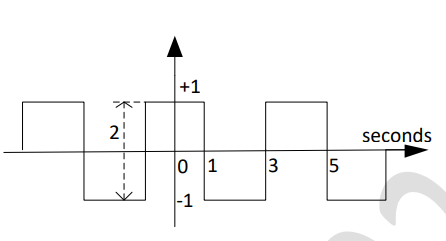
\includegraphics[width=0.4\columnwidth]{Figs/Fig 4.png}
\caption{periodicfunction}
\label{fig:placeholder}
\end{figure}
\hfill $\brak{GATE\ BM\ 2024}$

\item A cylindrical engineered tissue was developed with a diameter of 2 cm, height of 3 cm and Young's modulus of 20 MPa. If an axial tensile force of 10 N is applied, the percentage change in the height of the tissue is  \underline{\hspace{2cm}} \% .Give your answer
rounded off to 2 decimal places.\hfill $\brak{GATE\ BM\ 2024}$

\item The measured current through a device is 5 A, the voltage measured across the device is 20 V. The ammeter and the voltmeter used for these measurements have a measurement uncertainty of 1\% each. The maximum error in estimation of impedance of the device is\underline{\hspace{2cm}} m$\Omega$.Give your answer rounded to the nearest integer.\hfill $\brak{GATE\ BM\ 2024}$

\item The Larmor frequency of a Na nucleus when placed in a magnetic field strength of 3 T is  \underline{\hspace{2cm}} (The gyromagnetic ratio of Na is given as $\gamma$ = 11.26 MHz/T.)Give your answer in MHz rounded off to the nearest integer.\hfill $\brak{GATE\ BM\ 2024}$

\item A Doppler ultrasound transducer operating at 5 MHz gave maximum output frequency shift of 3 kHz. The velocity of sound in blood is 1500 m/s. If the probe was held at an angle of 45° to the direction of blood flow, the maximum velocity of blood flow through the artery is \underline{\hspace{2cm}}m/s. (Give your answer rounded off to two decimal places)
\begin{figure}[H]
\centering
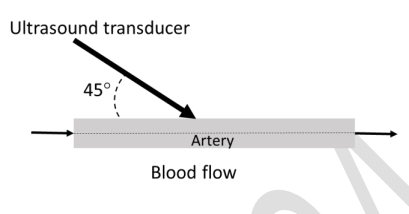
\includegraphics[width=0.4\columnwidth]{Figs/Fig 5.png}
\caption{ouypuyfrequency}
\label{fig:placeholder}
\end{figure}\hfill $\brak{GATE\ BM\ 2024}$

\item The wavelength of the peak emission from a human body at a temperature of $37^\circ\text{C}$
 due to black-body radiation is \underline{\hspace{2cm}} $\mu$m. The value of Wien's displacementconstant is 2.898 x $10^{-3}$ m K. (Give your answer rounded off to 2 decimal places.)\hfill $\brak{GATE\ BM\ 2024}$

 \item If 
\[
A = \begin{pmatrix}
1 & -1 \\
2 & -2
\end{pmatrix},
\]
the eigenvalues of $A$ are \underline{\hspace{2cm}}.
\begin{enumerate}[label=(\Alph*)]
    \item $-1 \text{ and } 0$
    \item $-1 \text{ and } +1$
    \item $-1 \text{ and } -1$
    \item $+1 \text{ and } 0$
\end{enumerate}
\hfill $\brak{GATE\ BM\ 2024}$

\item Consider a system of the following two partial differential equations:
\[
\frac{\partial \alpha}{\partial x} = -2 \frac{\partial \beta}{\partial t},
\quad
\frac{\partial \beta}{\partial x} = -2 \frac{\partial \alpha}{\partial t}.
\]

Which one of the following choices is a possible solution for the system?

\begin{enumerate}[label=(\Alph*)]
    \item $\alpha(t,x) = (x-t)^2 + (x+t)^2, \quad 
          \beta(t,x) = (x-t)^2 - (x+t)^2.$
          
    \item $\alpha(t,x) = (x-2t)^2 + (x+2t)^2, \quad 
          \beta(t,x) = (x-2t)^2 - (x+2t)^2.$
          
    \item $\alpha(t,x) = \left(x - \tfrac{t}{2}\right)^2 + \left(x + \tfrac{t}{2}\right)^2, \quad 
          \beta(t,x) = \left(x - \tfrac{t}{2}\right)^2 - \left(x + \tfrac{t}{2}\right)^2.$
          
    \item $\alpha(t,x) = \left(x - \tfrac{t}{2}\right)^2 + 2\left(x + \tfrac{t}{2}\right)^2, \quad 
          \beta(t,x) = 2\left(x - \tfrac{t}{2}\right)^2 - \left(x + \tfrac{t}{2}\right)^2.$
\end{enumerate}
\hfill $\brak{GATE\ BM\ 2024}$

\item The end-diastolic ventricular volume is found to be 125 mL and the end-systolic
ventricular volume is found to be 50 mL. If the heart rate is 65 beats/minute, what is
the cardiac output in liters per minute? (Rounded off to 2 decimal places.)
\begin{enumerate}[label=(\Alph*)]
    \item 3.25
    \item 4.88
    \item 5.20
    \item 3.00
\end{enumerate}
\hfill $\brak{GATE\ BM\ 2024}$

\item Which of the following waveforms represents the output V. of the circuit given
below? The Zener diode used has a Zener breakdown voltage of 1 V and can be
assumed ideal while in forward bias.
\begin{figure}[H]
\centering
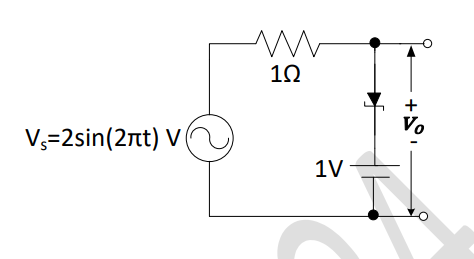
\includegraphics[width=0.6\columnwidth]{Figs/Fig 6.png}
\caption{breakdownvoltage}
\label{fig:placeholder}
\end{figure}
\begin{figure}[H]
\centering
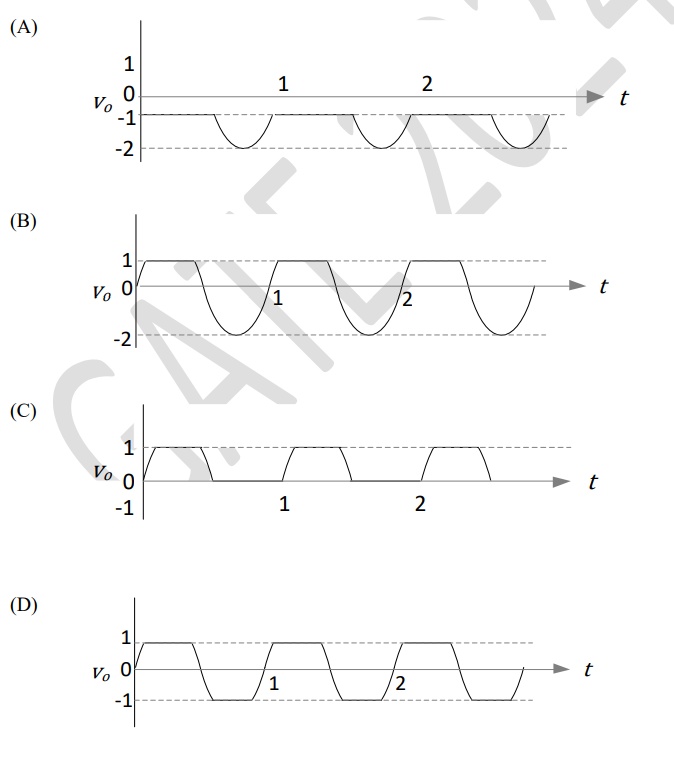
\includegraphics[width=0.8\columnwidth]{Figs/Fig 7.png}
\caption{waveforms}
\label{fig:placeholder}
\end{figure}

\item In magnetic resonance imaging (MRI), pulse repetition time ($TR$), time to echo ($TE$), $T_1$ relaxation time, $T_2$ relaxation time are some of the important pulse sequence design parameters. Which one of the following specifications is used for proton density weighted imaging?

\begin{enumerate}[label=(\Alph*)]
    \item \[
TR \gg T_1, \quad TE \ll T_2
\]

\item \[
TR \gg T_1, \quad TE \gg T_2
\]

\item \[
TR \ll T_1, \quad TE \ll T_2
\]

\item \[
TR \ll T_1, \quad TE \gg T_2
\]
\end{enumerate}
\hfill $\brak{GATE\ BM\ 2024}$

\item An orthopaedic implant when monitored over 6 months showed the following
normalized curves for polymer molecular weight (MW), mass of implant and
mechanical strength. Among the choices, what is the most probable reason for the
observed changes?
\begin{figure}[H]
\centering
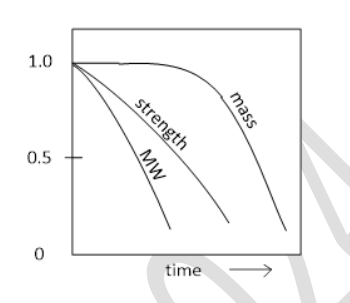
\includegraphics[width=0.4\columnwidth]{Figs/Fig 8.png}
\caption{curve}
\label{fig:placeholder}
\end{figure}
\begin{enumerate}[label=(\Alph*)]
    \item Bulk erosion
    \item Surface erosion
    \item Bulk initially followed by surface erosion
    \item No erosion but mechanical breakage due to injury
\end{enumerate}
\hfill $\brak{GATE\ BM\ 2024}$

\item In an attempt to integrate engineered tissue with native tissue, three samples of
engineered tissue, X, Y, Z, with identical material properties, were co-cultured
adjacent to three different native tissues (bone, cartilage and liver). The adhesive
strengths of X, Y, Z were observed after 8 weeks as follows.\\
\\Adhesive strength for X = 150 kPa, Y= 250 kPa, Z= 350 kPa\\
\\Match the native tissue that were used to co-culture X, Y and Z from the following.\\
\\I: Liver Tissue\\
II: Articular Cartilage\\
III: Devitalized Bone\\
\begin{enumerate}[label=(\Alph*)]
    \item X with I, Y with II and Z with III
    \item X with II, Y with III and Z with I
    \item X with I, Y with III and Z with II
    \item X with III, Y with II and Z with I
\end{enumerate}
\hfill $\brak{GATE\ BM\ 2024}$

\item In a catheter-sensor system to measure blood pressure (P) as shown in the below figure, the liquid resistance (RL) of the catheter is due to friction between shearing molecules flowing through the catheter. Which of the following is \textbf{TRUE} for RL if only the radius of the catheter is doubled. Assume that the pressure difference across the catheter segment is fixed.
\begin{figure}[H]
\centering
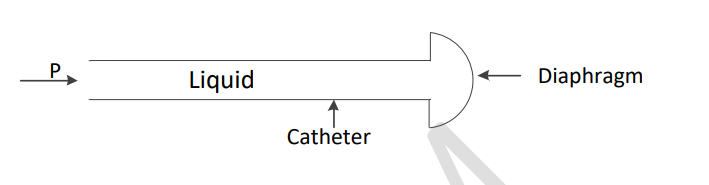
\includegraphics[width=0.4\columnwidth]{Figs/Fig 9.png}
\caption{radiography}
\label{fig:placeholder}
\end{figure}
\begin{enumerate}[label=(\Alph*)]
    \item RL will decrease by 16 times
    \item RL will decrease by 8 times
    \item RL will decrease by 4 times
    \item RL will decrease by 2 times
    \end{enumerate}
\hfill $\brak{GATE\ BM\ 2024}$

\item What is the value of the following integral using the residue integration method?

\[
\int_{-\infty}^{\infty} \frac{dx}{1+x^4}
\]

\begin{enumerate}[label=(\Alph*)]
    \item $\dfrac{\pi}{\sqrt{2}}$\\
    \item $\dfrac{\pi}{2\sqrt{2}}$\\
    \item $\dfrac{\pi}{4}$\\
    \item $\dfrac{\pi}{2}$\\
\end{enumerate}
\hfill $\brak{GATE\ BM\ 2024}$

\item A neurologist needs to observe the alpha wave in EEG recordings of a patient. The system block diagram with ideal filter blocks is shown below. Which one of the following design choices is correct?
\begin{figure}[H]
\centering
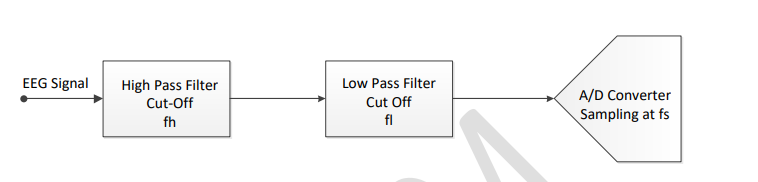
\includegraphics[width=0.8\columnwidth]{Figs/Fig 10.png}
\caption{wave}
\label{fig:placeholder}
\end{figure}
\begin{enumerate}[label=(\Alph*)]
    \item fh = 8 Hz, fl = 12 Hz, fs = 12 Hz
    \item fh = 4 Hz, fl = 6 Hz, fs = 24 Hz
    \item fh = 6 Hz, fl = 4 Hz, fs = 12 Hz
    \item fh = 8 Hz, fl = 12 Hz, fs = 48 Hz
\end{enumerate}
\hfill $\brak{GATE\ BM\ 2024}$

\item In the circuit below, what is the value of I1 to transfer the maximum power to load?
\begin{figure}[H]
\centering
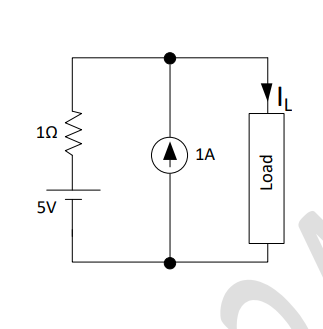
\includegraphics[width=0.4\columnwidth]{Figs/Fig 11.png}
\caption{circuit}
\label{fig:placeholder}
\end{figure}
\begin{enumerate}[label=(\Alph*)]
    \item 3A
    \item 6A
    \item 4A
    \item 2A
\end{enumerate}
\hfill $\brak{GATE\ BM\ 2024}$

\item A mechanical ventilator operating in volume controlled mode is set to deliver 600mL of tidal volume (TV) with a flow rate of 40 L/min. The frequency of breathing is set to 10 breaths per minute. If the flow rate is doubled which one of the following
\begin{enumerate}[label=(\Alph*)]
    \item The inspiratory time will increase.
    \item The expiratory time will increase.
    \item The tidal volume will increase.
    \item The frequency of breathing will decrease.
\end{enumerate}
\hfill $\brak{GATE\ BM\ 2024}$

\item The X-ray attenuation coefficients as a function of photon energy for three materials are shown in the figure below. A tissue phantom containing these three materials is imaged at two different X-ray photon energies of 50 keV and 150 keV. When the developed X-ray film is viewed, which of the following statements is/are \textbf{TRUE}?
\begin{figure}[H]
\centering
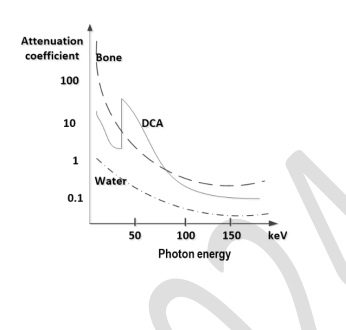
\includegraphics[width=0.4\columnwidth]{Figs/Fig 14.png}
\caption{radiography}
\label{fig:placeholder}
\end{figure}
\begin{enumerate}[label=(\Alph*)]
    \item bone will appear relatively brighter than DCA in 50 keV.
    \item DCA will appear relatively brighter than bone in 50keV.
    \item Bone will appear relatively brighter than DCA in 150 keV.
    \item DCA will appear relatively brighter than bone in 150 keV.
\end{enumerate}
\hfill $\brak{GATE\ BM\ 2024}$

\item Which of the following is/are TRUE for a surface electromyography (sEMG) signal
of a muscle experiencing fatigue?
\begin{enumerate}[label=(\Alph*)]
\item  The median frequency of power spectral density of sEMG will decrease.
\item  The median frequency of power spectral density of sEMG will increase.
\item The root mean square (RMS) value of sEMG will increase.
\item The root mean square (RMS) value of sEMG will decrease.
\end{enumerate}
\hfill $\brak{GATE\ BM\ 2024}$

\item For $\vec{F} = (x+y)\hat{i} + (x+y)\hat{j}$ the value of 
\[
\oint \vec{F} \cdot d\vec{r}
\]
along the path shown in the figure is  \underline{\hspace{2cm}}. Give your answer as an integer.
\begin{figure}[H]
\centering
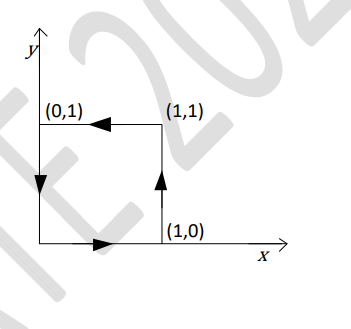
\includegraphics[width=0.4\columnwidth]{Figs/Fig 12.png}
\caption{path}
\label{fig:placeholder}
\end{figure}

\item The approximate total cross sectional areas of various types of blood vessels are given below. It was estimated that the velocity of blood in the aorta is $30 \,\text{cm s}^{-1}$. The time it will take for the blood to travel through a capillary of length $0.5 \,\text{mm}$ is \_\_\_\_\_ seconds. Give your answer rounded off to two decimal places.

\bigskip

\begin{center}
\begin{tabular}{|c|c|}
\hline
\textbf{Vessel Type} & \textbf{Approximate total cross sectional area (cm$^2$)} \\
\hline
Aorta      & 4.5  \\
\hline
Artery     & 20   \\
\hline
Arteriole  & 400  \\
\hline
Capillary  & 4500 \\
\hline
Venule     & 40   \\
\hline
Vein       & 15   \\
\hline
\end{tabular}
\end{center}
\hfill $\brak{GATE\ BM\ 2024}$


\item A DNA extract solution with a concentration of 15 ng/$\mu$L placed in a micro-cuvette of
sample thickness 0.5 mm gave an absorbance of 0.24 at a wavelength of 260 nm in a
spectrophotometer. After further concentration, the sample was found to give an
absorbance of 0.38 at the same wavelength under identical conditions. The final
concentration of the sample is \underline{\hspace{2cm}}ng/$\mu$L. (Give your answer rounded off to 2 decimal places)\hfill $\brak{GATE\ BM\ 2024}$

\item An X-ray beam of initial intensity Io of 70 keV imaging the chest is assumed to undergo
attenuation through the muscle tissue for a thickness of 16 cm and further through the
bone tissue for a thickness of 4 cm. The half value layer (HVL) thicknesses for the
muscle and bone are 3.5 cm and 1.8 cm, respectively. The percentage of X-ray
intensity transmitted through the body is\underline{\hspace{2cm}}
 Give your answer rounded off to 2 decimal places.\hfill $\brak{GATE\ BM\ 2024}$

\item A person standing one meter away from a 4000 curie radioactive source receives a
lethal dose of radiation in about 5 minutes. At 3 meters away from the same source,
the time in which he will receive the same lethal dose is \underline{\hspace{2cm}}
minutes. Give your answer rounded off to the nearest integer.\hfill $\brak{GATE\ BM\ 2024}$

\item If a circular ultrasound transducer of radius $a = 8 \,\text{mm}$ operating at a central frequency of $1 \,\text{MHz}$ has a pressure beam pattern in a medium as given below:
\[
P(r,0) \propto \sin \left(\frac{ka^2}{4r}\right)
\]

Here, $k$ is the wave number, $r$ is the axial distance from the center of aperture. The speed of sound in the medium is $1600 \,\text{ms}^{-1}$.

\bigskip

The reduction in intensity between $r = 8 \,\text{cm}$ and $r = 16 \,\text{cm}$ is \underline{\hspace{2cm}} dB. Give your answer as a positive quantity rounded off to two decimal places.
\hfill $\brak{GATE\ BM\ 2024}$

\item The source in the figure is a current source and the circuit is in steady state. At t =
0.5$\pi$ seconds, the value of v in the circuit given below is \underline{\hspace{2cm}} volts. Give your answer rounded off to 2 decimal digits.
\begin{figure}[H]
\centering
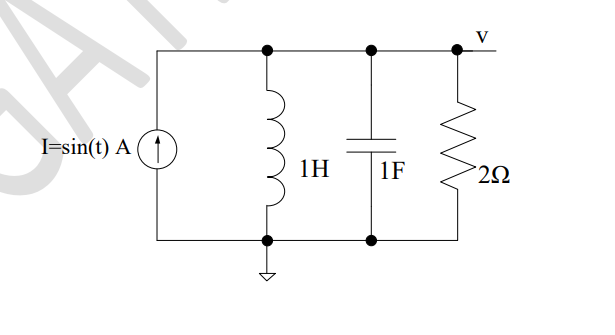
\includegraphics[width=0.4\columnwidth]{Figs/Fig 13.png}
\caption{currentsource}
\label{fig:placeholder}
\end{figure}\hfill $\brak{GATE\ BM\ 2024}$

\item The equivalent impedance, $Z_{AB}$, in the circuit given below is
\underline{\hspace{2cm}}~$\Omega$. Give your answer rounded off to one
decimal place.
\begin{figure}[H]
\centering
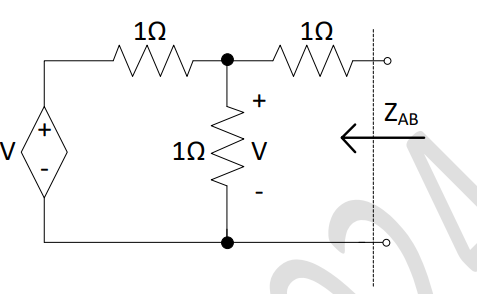
\includegraphics[width=0.4\columnwidth]{Figs/Fig 15.png}
\caption{impedence}
\label{fig:placeholder}
\end{figure}\hfill $\brak{GATE\ BM\ 2024}$

\item The bandwidth of ECG signal ranges from 0.5 Hz to 100 Hz. If a single ADC is used to digitize data from 8 ECG channels then the minimum ADC sampling rate is\underline{\hspace{2 cm}}Hz. Give your answer rounded off to the nearest integer.\hfill $\brak{GATE\ BM\ 2024}$

\item If $x[n] = u[n] - u[n-5]$, and $h[n] = \delta[n] - \delta[n-1]$ and 
$y[n] = x[n] * h[n]$, then the value of 
$\sum_{n=-\infty}^{\infty} y[n]$ is \underline{\hspace{2cm}}. 
Give your answer rounded off to the nearest integer.\hfill $\brak{GATE\ BM\ 2024}$

\item In the figure below, the diode is ideal. The current reading shown in the ammeter is \underline{\hspace{2cm}}A. Give your answer rounded off to the nearest integer.
\begin{figure}[H]
\centering
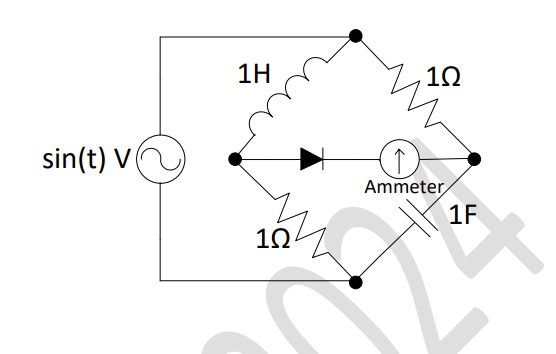
\includegraphics[width=0.4\columnwidth]{Figs/Fig 16.png}
\caption{currentreading}
\label{fig:placeholder}
\end{figure}\hfill $\brak{GATE\ BM\ 2024}$

\item In the figure below, the Fourier series of $v(t)$, in volts, is given as:  

\[
v(t) = v_0 + 2 \cos(\omega_0 t) + 5 \cos(3\omega_0 t) + \cos(5\omega_0 t)
\]

The capacitor is a short circuit for all AC signals. The power absorbed by the 
$1 \, \Omega$ resistor is \underline{\hspace{1.2cm}} W.  
Give your answer rounded off to the nearest integer.
\begin{figure}[H]
\centering
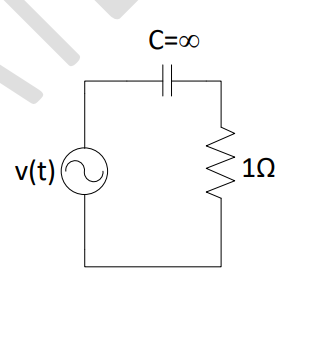
\includegraphics[width=0.4\columnwidth]{Figs/Fig 17.png}
\caption{series}
\label{fig:placeholder}
\end{figure}\hfill $\brak{GATE\ BM\ 2024}$

\item An artificial fore-arm has a moment-of-inertia around the center of mass as 0.3kg.$m^2$.
The mass of the artificial fore-arm is 3 kg. If the distance from the elbow joint to the
center of mass of the fore-arm is 20 cm, the moment-of-inertia of the fore-arm about the elbow joint is \underline{\hspace{1.2cm}}kg.$m^2$. Give your answer rounded off to two decimal places.\hfill $\brak{GATE\ BM\ 2024}$

\item A bio-potential signal of 4 mV on the skin surface was fed to an amplifier with a
differential gain of 2000. The noise in the signal is 1000 mV. If the amplifier output
produces a noise output of 200 mV, the common mode rejection ratio of the amplifier is \underline{\hspace{1.2cm}}
dB. Give your answer rounded to the nearest integer.\hfill $\brak{GATE\ BM\ 2024}$

\item In a motor nerve conduction velocity experiment, the distance between the distal and
the recording sites is 4 cm and the distance between the proximal and the recording
sites is 24 cm. The distal and proximal latencies were recorded as 6 ms and 10 ms,
respectively. The nerve conduction velocity is\underline{\hspace{1.2cm}}meters per second. Give your is
answer\hfill $\brak{GATE\ BM\ 2024}$

\item A person creates an apparatus as shown in the figure to exercise the extensor muscle 
of the hand. It is given that $OP = 0.15 \, \text{m}$, $OQ = 0.35 \, \text{m}$, 
$\theta = 30^\circ$, the weight of the lower arm $= 20 \, \text{N}$, the center 
of mass of the lower arm is at point $P$, the magnitude of the applied tensile force 
$F = 50 \, \text{N}$. If the extensor muscle is acting with a moment arm of 
$0.25 \, \text{m}$, the muscle force required to hold the hand at the position shown 
in the figure is \underline{\hspace{1.2cm}} N. Give your answer rounded off to the nearest integer.
\begin{figure}[H]
\centering
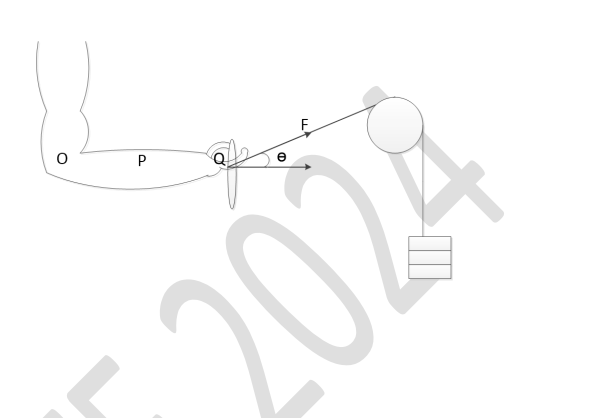
\includegraphics[width=0.4\columnwidth]{Figs/Fig 18.png}
\caption{picture}
\label{fig:placeholder}
\end{figure}\hfill$\brak{GATE\ BM\ 2024}$



\end{enumerate}
\end{document}
